\section{Proposed Architecture}\label{Architecture}

\subsection{Overview}\label{Network}
Here we discuss overall architecture of the proposed load balancer.
\begin{figure}
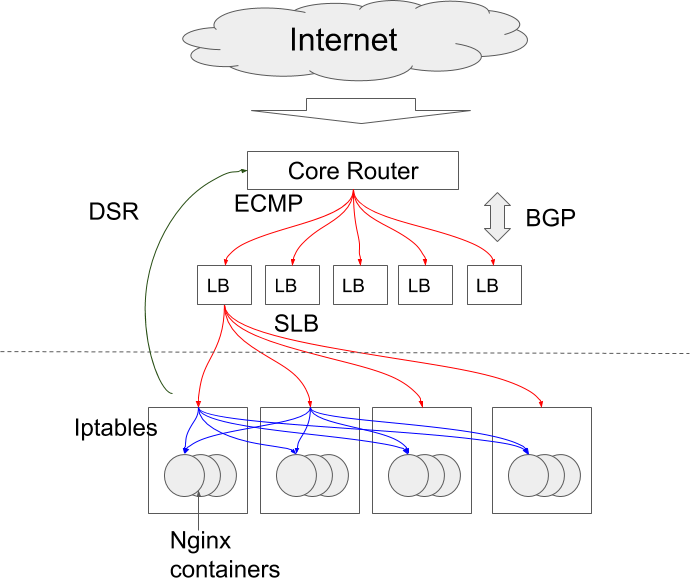
\includegraphics[width=\columnwidth]{Figs/google_lb}
\caption{Conventional architecture. Software load balancers are set up via cloud API. }
\label{fig:google_lb}
\end{figure}
Figure~\ref{fig:google_lb} show conventional architecture of the container cluster infrastructure, e.g. Kubernetes.
Below the dotted line, there are node Linux machines that hosts containers, which is controlled by Kubernetes.
Above the dotted line, there are Software Load Balancers(SLBs) and the core router.
All the equipment and software entities above the dotted line are controlled by base cloud infrastructure.

Upon launch of the container clusters, SLBs are set up by the cloud infrastructure.
At the same time iptables DNAT rule's are set up on each of the node Linux machines.
These SLBs distribute incoming traffic to every node that hosts containers.
The traffic is then distributed again to destination containers using iptables destination 
network address translation (DNAT)\cite{MartinA.Brown2017,Marmol2015} rules in a round-robin manner. 

\begin{figure}
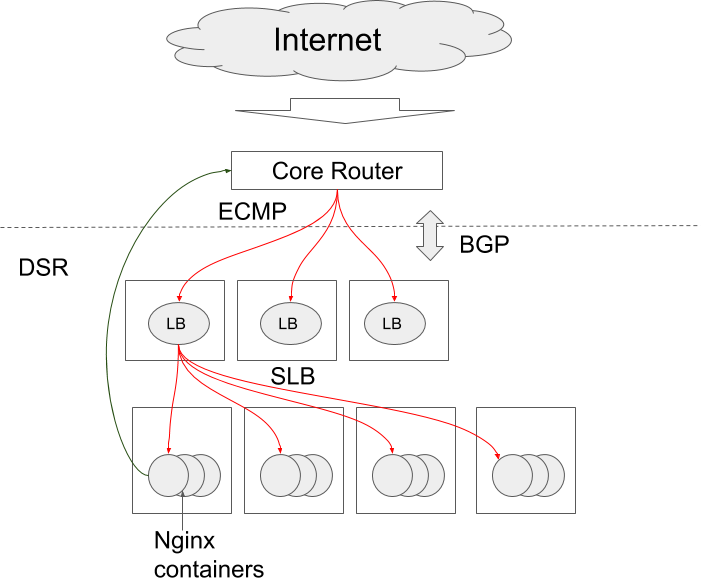
\includegraphics[width=\columnwidth]{Figs/new_lb}
\caption{Proposed architecture. Routing table of the Core Router is updated via BGP.}
\label{fig:new_lb}
\end{figure}

Figure~\ref{fig:new_lb} shows proposed architecture.
Upon launch of the container clusters, SLBs are also launched as a part of the container cluster.
Then, the SLBs communicate with the Core router using the Border Gateway Protocol(BGP)\cite{rekhter2005border} to update routing table.
The core router evenly distributes the incoming traffic to SLBs, then the SLB directly forward the traffic to destination containers.

The big differences between the conventional architecture and the proposed ones are;
a) iptables DNAT load balancing layer does not exist in the latter,
b) while the communication between the Kubernetes and the cloud provider in the conventional architecture is the vendor specific API requests to setup the external SLBs, the communication between the Kubernetes and the cloud provider is standard BGP protocol in the proposed architecture.

In other words, the proposed architecture is better than the conventional one, because it eliminates one extra network hop and communicate with external world using standard protocol.
And also because the SLBs are containerized and are the part of the cluster, a service can be deployed in any environment including on-premise data centers, if only the core router permits the update of its routing table via BGP.
This will greatly improve the portability compared to the conventional architecture where the support for vendor specific API is always required.

